\section{Logit models}\label{sec:loglin-logit}
Because \loglin\ models are  formulated as models for the
log (expected) frequency, they make no distinction between
response and explanatory variables.
In effect, they treat all variables as responses.
Logit models, on the other hand,
describe how the log odds for one variable depends on other,
explanatory variables.
There is a close connection between the two:
When there is a response variable, each logit model for that response
is equivalent to a \loglin\ model.
This relationship often provides a simpler way to formulate and test
the model, and to plot and interpret the fitted results.
The price paid for this simplicity is that associations among the
explanatory variables are not expressed in the model.

Consider, for example, the model of homogeneous association,
\eqref{eq:lno3way} for a three-way table, and let variable $C$
be a binary response.  Under this model, the logit for variable $C$
is
\begin{eqnarray*}
  L_{ij}  =
  \log \left(  \frac{\pi_{ij|1}}{\pi_{ij|2}} \right) & = &
  \log \left(  \frac{m_{ij1}}{m_{ij2}} \right) \\
    &  = &
  \log (m_{ij1}) - \log (m_{ij2})
  \period
\end{eqnarray*}
Substituting from \eqref{eq:lno3way}, we find that all terms which do not
involve variable $C$ cancel, and we are left with

\begin{eqnarray} \label{eq:logitab1}
  L_{ij}  =
  \log ( m_{ij1} /  m_{ij2} )  & = &
  ( \lambda_1^C - \lambda_2^C )  +
  ( \lambda_{i1}^{AC} - \lambda_{i2}^{AC} )  +
  ( \lambda_{j1}^{BC} - \lambda_{j2}^{BC} )  \nonumber \\
  &  = &
  2 \lambda_1^C   +   2 \lambda_{i1}^{AC} +   2 \lambda_{j1}^{BC}
\end{eqnarray}
because all \(\lambda\) terms sum  to zero.  We are interested in how these
logits depend on $A$ and $B$, so we may replace the $\lambda$ parameters
with new parameters,
 \(\alpha  = 2
\lambda_1^C\), \(\beta _i^A = 2 \lambda_{i1}^{AC}\), etc., which express this relation more directly,
\begin{equation}\label{eq:logitab2}
  L_{ij}  =
  \alpha   +  \beta _i^A +  \beta _j^B
  \period
\end{equation}
In the logit model \eqref{eq:logitab2}, the response, $C$, is affected
by both $A$ and $B$, which have additive effects on the log odds of response
category $C_1$ compared to $C_2$.
The terms $\beta _i^A$ and  $\beta _j^B$
correspond directly to $[AC]$ and $[BC]$ in the \loglin\ model \eqref{eq:lno3way}. The association among the explanatory variables,
$[AB]$ is assumed in the logit model, but this model provides no explicit
representation of that association.  The logit model \eqref{eq:logitab1}
is equivalent to the \loglin\ model $[AB] [AC] [BC]$ in goodness-of-fit
and fitted values, and parameters in the two models correspond directly.

More generally, when there is a binary response variable, say $R$, and
one or more explanatory variables, $A, B, C, \dots$, any logit model
for $R$ has an equivalent \loglin\ form.
Every term in the logit model, such as $\beta_{ik}^{AC}$, corresponds to
an association of those factors with $R$, that is, $[ACR]$ in the
equivalent \loglin\ model.  The \loglin\ model must also include all
associations among the explanatory factors, the term $[A B C \dots]$.
Conversely, any \loglin\ model which includes all associations among
the explanatory variables has an equivalent logit form.
When the response factor has more than two categories, models for
generalized logits have equivalent \loglin\ form.

\begin{Example}[berkeley7]{Berkeley admissions}
The homogeneous association model, $[AD] [AG] [DG]$
did not fit the Berkeley admissions data very well,
and we saw that the term $[AG]$ was unnecessary.
Nevertheless, it is instructive to consider the equivalent logit model.
We illustrate the features of the logit model which lead to the same
conclusions and simplified interpretation from graphical displays.

Because Admission
is a binary response variable, model \eqref{eq:berk1} is equivalent
to the logit model,

\begin{equation}\label{eq:berk3}
  \log \left(
  \frac{m_{ \mbox{\scriptsize{Admit}} (ij) }} {m_{ \mbox{\scriptsize{Reject}} (ij) }}
  \right)
  =
  \alpha   +  \beta _i^{\mbox{\scriptsize Dept}}
  +  \beta _j^{\mbox{\scriptsize Gender}}
  \period
\end{equation}
That is, the logit model \eqref{eq:berk3} asserts that department and
gender have additive effects on the odds of admission.
This model may be fit with \PROC{CATMOD}
as shown below, using the variable \pname{admit} as the response
and \pname{dept} and \pname{gender} as predictors.
The option \pname{order=data} is used so that \PROC{CATMOD} will
form the logit for 'Admitted', the category which appears first
in the \Dset.
The \stmt{RESPONSE}{CATMOD} is used
to create an \ODS\
containing observed and fitted logits, which are graphed
(see \exref{ex:berkeley8}) in
\figref{fig:catberk2}.

\begin{listing}
proc catmod order=data
            data=berkeley;
   weight freq;
   response / out=predict;
   model admit = dept gender / ml noiter noprofile ;
\end{listing}

The model fit statistics and parameter estimates for the model
\eqref{eq:berk3} are shown in \outref{out:catberk2.1}.
Note that the \LR\ \GSQ\ for this model is the same as
that for the \loglin\ model $[AD][AG][DG]$
shown in \outref{out:catberk5.1} and in \outref{out:genberk2.1}
and the Wald \chisq\ values for \pname{dept} and \pname{gender}
in \outref{out:catberk2.1}
are similar to the \chisq\ values for the association of each
of these with \pname{admit}
in the \loglin\ model.

\begin{Output}[htb]
\caption{Berkeley admissions data, fit statistics and parameter estimates for the logit model \eqref{eq:berk3}}\label{out:catberk2.1}
\small
\verbatiminput{ch7/out/catberk2.1}
\end{Output}

As in logistic regression models, parameter estimates may be interpreted
as increments in the log odds, or $\exp(\beta)$ may be interpreted
as the multiple of the odds associated with the explanatory categories.
Because \PROC{CATMOD} uses zero-sum constraints,
$\sum \beta_i^{\mbox{\scriptsize   Dept}} =0$ and
$\sum \beta_j^{\mbox{\scriptsize   Gender}} =0$, the parameters for the
last level of any factor
is found as the negative of the sum of the parameters listed.

Thus, $\beta_1^{\mbox{\scriptsize   Gender}} = -0.0499$
is the increment to the log odds of admission for men,%
\footnote{$\beta_1^{\mbox{\scriptsize   Gender}}$ refers to
the first level of \pname{gender} to appear in the \pname{berkeley}
\Dset, because \pname{order=data} was used on the \PROC{CATMOD} statement.}
and therefore $\beta_2^{\mbox{\scriptsize Gender}} = +0.0499$ for women.
Overall, but controlling for department, women were $\exp(2 \times 0.0499) = 1.105$
times as likely to be admitted to graduate school than male applicants
in 1973.
The logit parameters for \pname{dept} in \outref{out:catberk2.1} decrease
over departments A--E; the value for department F is $-(1.274 + 1.231 + \cdots
-0.465) = -2.032$.
These values correspond to the decline in the fitted logits
over department seen in \figref{fig:catberk2}.

Logit models are easier to interpret than the corresponding \loglin\
models because there are fewer parameters,
and because these parameters pertain to the odds of a response category
rather than to cell frequency.
Nevertheless, interpretation is often easier still from a graph than from the
parameter values.
\end{Example}


\subsection{Plotting results for logit models}

Logit models may also be interpreted through plots of observed and
fitted values, either in terms of the logit for one response category
or in terms of the equivalent response probability.
Plots of log odds generally have a simpler, additive form, such as
the parallel curves in \figref{fig:catberk2},
but the effects may be easier to understand in terms of
probabilities.
As with logistic regression models, both goals may often be
achieved by plotting on the logit scale and adding a second vertical
axis showing the corresponding probabilities.
These plots are similar to those described in \secref{sec:logist-quant}
and \secref{sec:logist-qual}, but the plotting steps differ because
the output information from \PROC{CATMOD} is structured differently
from that provided by \PROC{LOGISTIC}.

Such plots are facilitated by the \macro{CATPLOT} (\macref{mac:catplot}).
The macro uses the \ODS\  produced with the \pname{OUT=} option on the \stmt{RESPONSE}{CATMOD}.
This \Dset\ normally contains both logit values
and probability values, and either type may be plotted, with observed
and fitted values, and optional confidence intervals.
A utility macro, \pname{PSCALE} (\macref{mac:pscale}) may be used to add a probability scale
to a plot of log odds.
\begin{Example}[berkeley8]{Berkeley admissions}
The \ODS\ \pname{predict} from the logit model, \pname{admit = dept gender},
for the Berkeley data is shown partially in \outref{out:catberk2.2}.
Each of the $ 2 \times 6$ samples defined by the explanatory factors
\pname{dept, gender}
gives rise to three observations: two response probabilities and
one logit, distinguished by the variable \verb|_TYPE_|.
\begin{Output}[htb]
\caption{Output \Dset\ \pname{predict} from the logit model for Berkeley admissions (partial)}\label{out:catberk2.2}
\small
\verbatiminput{ch7/out/catberk2.2}
\end{Output}

%% one figure
\begin{figure}[htb]
  \centering
  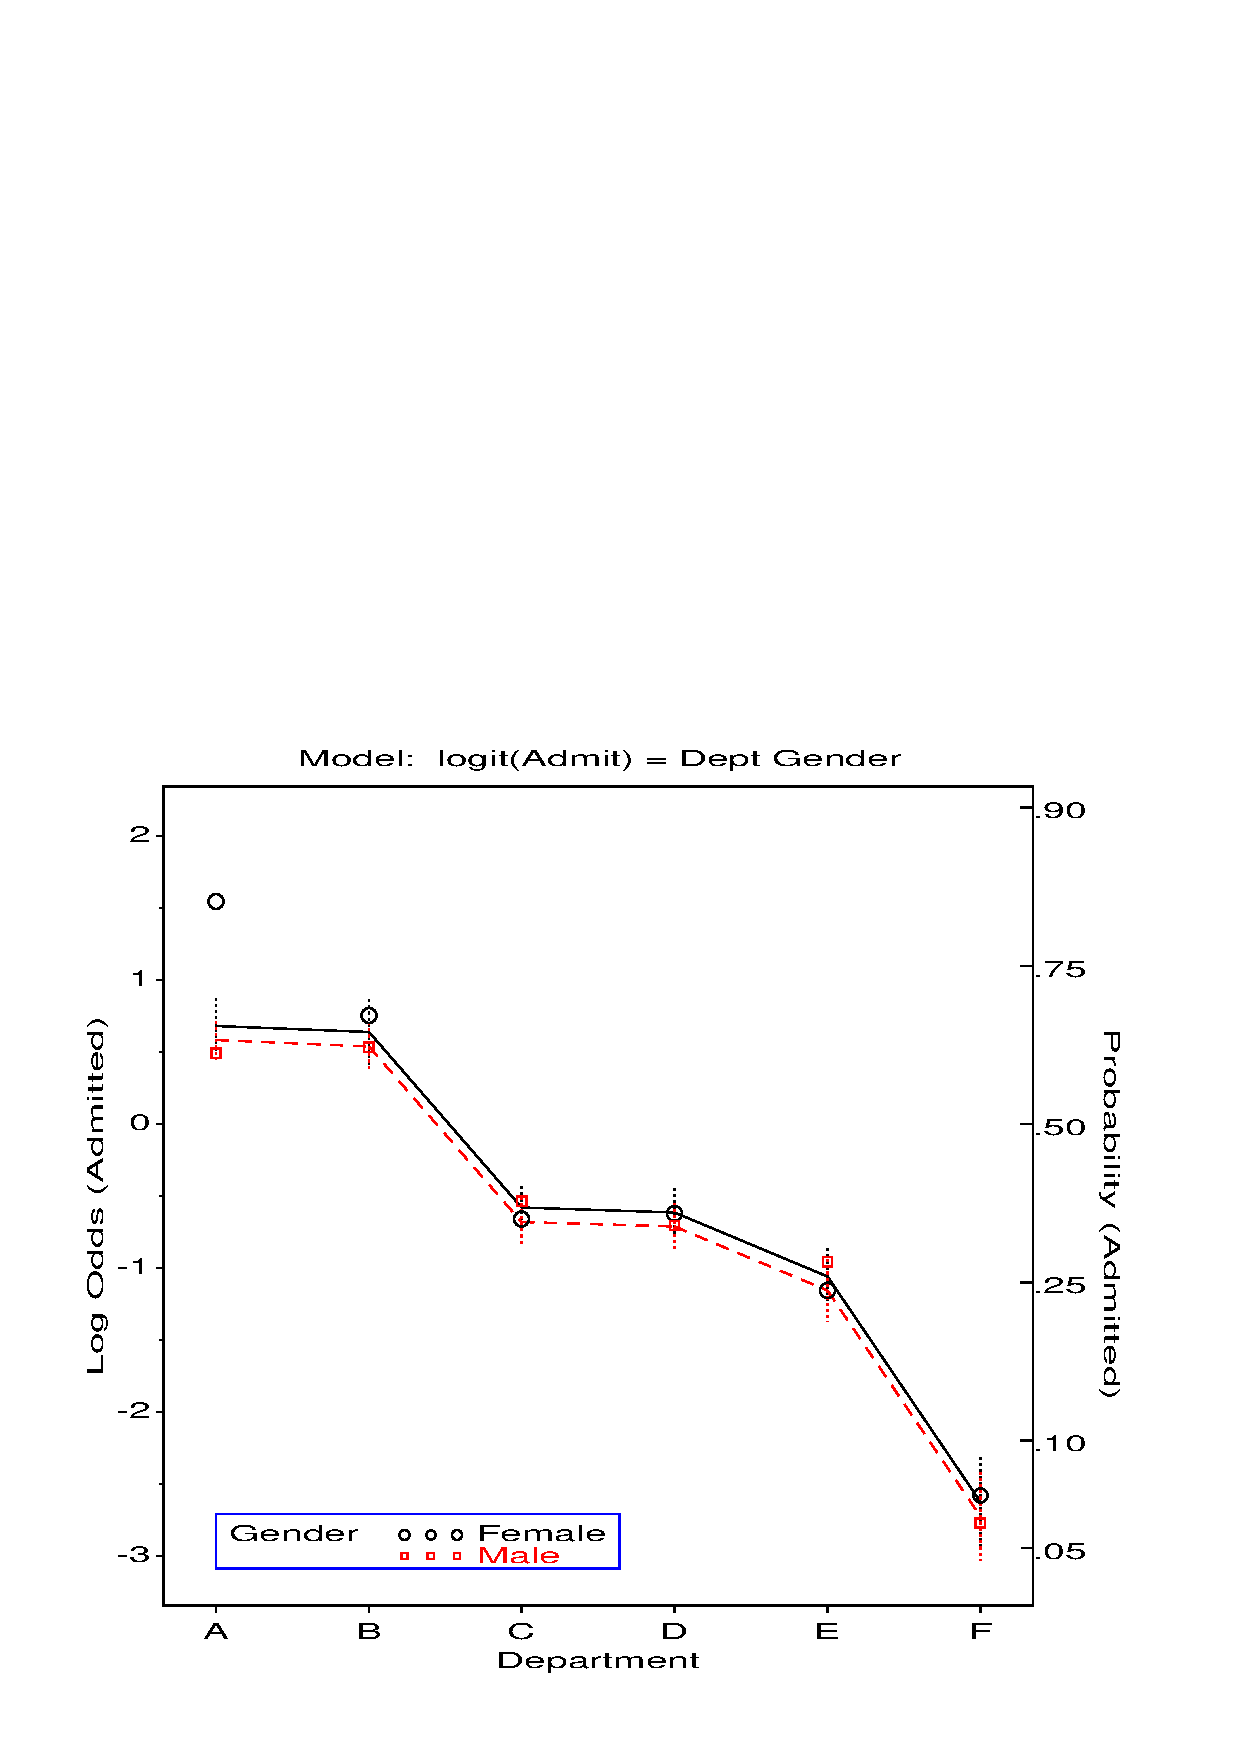
\includegraphics[scale=.6]{catberk2}
  \caption[Observed and fitted log odds of admission in the logit model]{Observed (points) and fitted (lines) log odds of admission in the logit model
  corresponding to [AD][AG][DG].  The error bars show individual 95\%
  confidence intervals around each fitted logit.}%
  \label{fig:catberk2}
\end{figure}

The statements below draw the plot of observed and predicted logits
(\verb|_type_='FUNCTION'|) shown in \figref{fig:catberk2}.
The \macro{PSCALE} constructs an \ADS\
which draws the probability values on the right vertical axis in the
plot.
The label for this axis is specified in the \stmt{TITLE}{GPLOT}, with
an angle, \pname{A=-90}, meaning the right-hand side, rotated \degree{90}.
By default, the macro uses the \pname{AXIS} and \pname{SYMBOL}
statements defined before the macro call.
Separate curves are
drawn for each level of the \pname{CLASS=GENDER} variable.
The values of the \pname{CLASS} variable may be labeled in the plot
or supplied in a \stmt{LEGEND}{CATPLOT}.
The parameter \pname{Z=1.96} specifies the multiple of
the standard error of the fitted logit (\verb|_SEPRED_|) used to
draw the error bars in the plot,
giving (asymptotic) 95\% individual confidence intervals.
\begin{listing}
%pscale(lo=-4, hi=3, anno=pscale, prob=%str(0.05,.1,.25,.5,.75,.9));

title h=1.6 'Model:  logit(Admit) = Dept Gender'
            a=-90 'Probability (Admitted)'
      h=3.5 a=-90 ' ';
legend1 position=(bottom inside left)  offset=(4,3)
        mode=share cborder=blue across=1
        shape=symbol(6,1.5) label=('Gender')
        value=(c=black 'Female'
               c=red   'Male');
axis1 order=(-3 to 2) offset=(4)
      label=(a=90 'Log Odds (Admitted)');
axis2 label=('Department') offset=(4);
symbol1 i=none v=circle h=1.7 c=black;
symbol2 i=none v=dot    h=1.7 c=red  ;
%catplot(data=predict,
   xc=dept, y=_obs_, class=gender,
   type=FUNCTION,
   z=1.96, anno=pscale, legend=legend1);
\end{listing}

The effects seen in our earlier analyses (Examples~\ref{ex:berkeley4}
and \ref{ex:berkeley4b})
may all be observed in this
plot.
The effect of gender is shown by the constant separation
between the two curves.
From the plot we see that this effect is very small and nonsignificant (compared
with the error bars).
If the gender effect were omitted from the model,
the fitted logits would be the same
for men and women applying to each department, and would plot as a curve
parallel to, but in between, the two shown in the graph.
Most of the observed points are quite close to their predicted values,
except in Department A,
where the probability of admittance for women is substantially
greater than that for men.
In \exref{ex:berkeley6} we dealt with this by allowing one extra parameter
for an association between admission and gender in department A,
giving the \loglin\ model \eqref{eq:berk2}.

We can see what this model ``looks like'' by recasting it in logit form.
The \loglin\ model \eqref{eq:berk2}
has an equivalent logit formulation, which also adds a 1 df term for an
effect of gender in department A,
\begin{equation}\label{eq:berk4}
  L_{ij} =
  \alpha   +  \beta _i^{\mbox{\scriptsize Dept}}
  +  \delta_{j=1} \beta^{\mbox{\scriptsize Gender}}
  \period
\end{equation}

This model may be fit
with \PROC{CATMOD} as shown below.  The association term between admission
and gender for Dept. A (\texttt{dept1AG}) is fit as a \pname{DIRECT}
variable.  The \pname{gender} variable is not included in the
\stmt{MODEL}{CATMOD}, so it must be listed in the
\stmt{POPULATION}{CATMOD}.
Because the \macro{CATPLOT}
uses the values in the \ODS, the plotting step is unchanged.

\begin{listing}
data berkeley;
   set berkeley;
   dept1AG = (gender='F') * (dept=1);

proc catmod order=data
            data=berkeley;
   weight freq;
   population dept gender;
   direct dept1AG;
   response / out=predict;
   model admit = dept dept1AG / ml noiter noprofile ;
%catplot(data=predict, xc=dept, class=gender, type=FUNCTION,
   z=1.96, legend=legend1);
\end{listing}

%% one figure
\begin{figure}[htb]
  \centering
  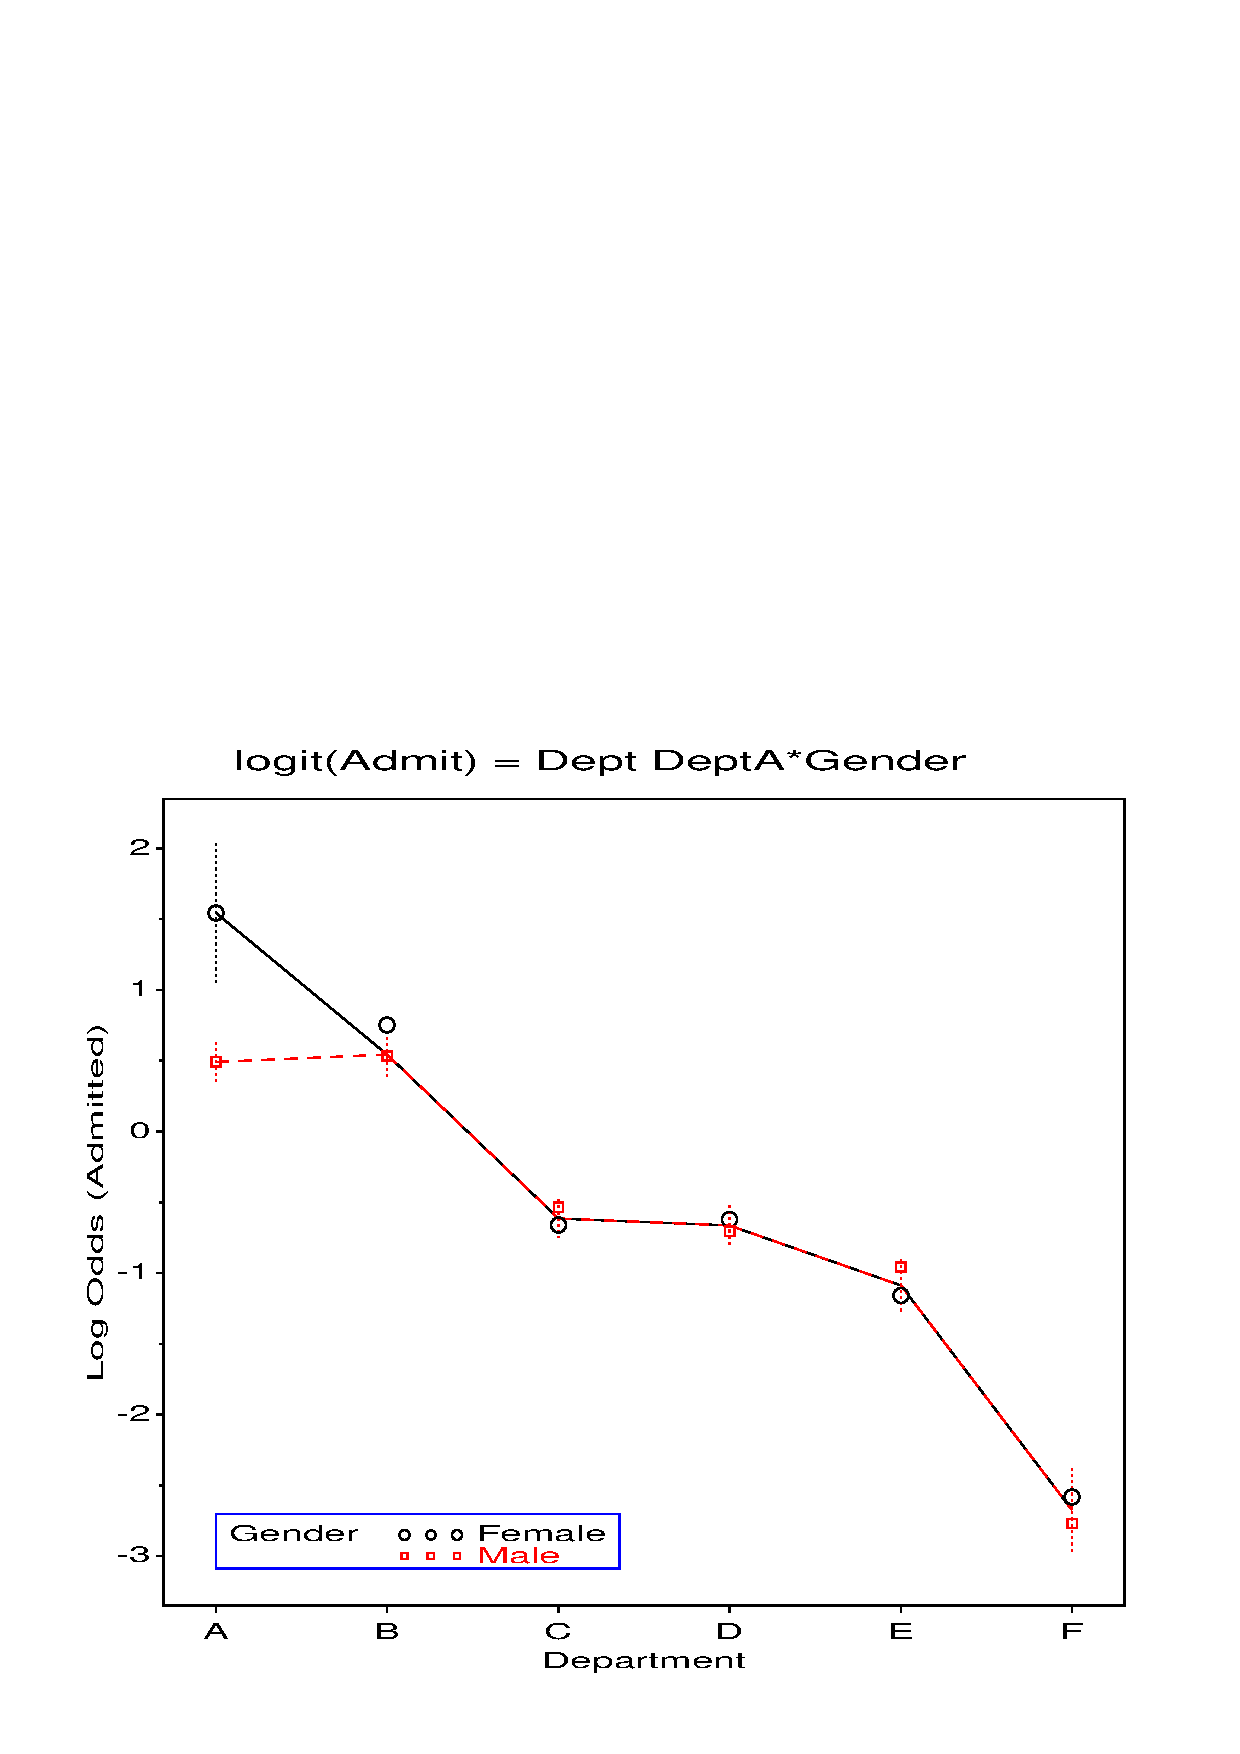
\includegraphics[scale=.6]{catberk6}
  \caption{Observed and fitted logits for model \eqref{eq:berk2}}%
  \label{fig:catberk6}
\end{figure}
The resulting plot for this model is shown in \figref{fig:catberk6}.
The graph gives a visual interpretation of the model
\eqref{eq:berk2} and its logit form, \eqref{eq:berk4}:
No effect of gender on admission, except in department A, where the
extra parameter allows perfect fit.
\end{Example}


\subsection{Zero frequencies}
Cells with frequencies of zero create problems for \loglin\ and logit
models.  For \loglin\ models, most of the derivations of expected
frequencies and other quantities assume $n_{ijk\cdots} > 0$.
In logit models, the observed log odds (e.g., for a three-way table),
$\log ( n_{ij1} / n_{ij2} )$, will be undefined if either frequency is
zero.

Zero frequencies may occur in \ctabs\ for two different reasons:
\begin{description}
\item[structural zeros] (also called \emph{fixed zeros}) will occur when it is impossible to observe
values for some combinations of the variables.
For example, suppose we have three different methods of contacting
people at risk for some obscure genetically inherited disease:
newspaper advertisement, telephone campaign, and radio appeal.
If each person contacted in any way is classified dichotomously
by the three methods of contact, there can never be a non-zero
frequency in the `No-No-No' cell.%
\footnote{Yet, if we fit an unsaturated model, expected frequencies
may be estimated for all cells, and provide a means to estimate
the total number at risk in the population.
See \citet[Section 5.4]{Lindsey:95}.}
\item[sampling zeros] (also called \emph{random zeros})
occur when the total size of the sample is not large enough in relation to the probabilities in each of the cells to assure that someone will be observed
in every cell.
For example, in a European survey of religious affiliation and occupation,
we may not happen to observe any Muslim vineyard-workers in France, although such individuals surely exist.
Even when zero frequencies do not occur, tables with many cells relative to
the total frequency tend to produce small expected frequencies in at
least some cells, which tends to make  the \chisq\ statistics for model fit
and Wald statistics for individual terms unreliable.
\end{description}

\PROC{CATMOD} takes a simple approach to distinguishing these two cases:
Cells with zero frequency are simply deleted from the \ctab,
and thus are treated as structural zeros.  To avoid this, some corrective
action is needed.
One solution (for sampling zeros) is to collapse categories of some variables,
but we are often loath to do this for fear of loss of information.

Other suggestions are:
\begin{seriate}
\item Add a small positive quantity (0.5 is usually recommended) to every
cell in the \ctab\ \citep{Goodman:70}, as is done in calculating
empirical log odds (\secref{sec:logist-logodds});
\PROC{CATMOD} provides the \opt{ADDCELL}{CATMOD} in the \stmt{MODEL}{CATMOD} for this purpose,
but this option is ignored for maximum likelihood estimation.
\item Replace sampling zeros by some small number, typically
$10^{-10}$ or smaller \citep{Agresti:90}.
\item Add a small quantity, like 0.1, to all zero cells
\citep{EversNamboodiri:77}.
\end{seriate}

\begin{Example}[reagan]{Race and politics in the 1980 US Presidential vote}
\tabref{tab:reagtab} shows data (\citet[Table 4.12]{Agresti:90}, from \citet{CloggShockey:88})
from the 1982 General Social Survey on
votes in the 1980 US Presidential election for Reagan or for Carter
or other in relation to race and conservatism (1=most liberal,
7=most conservative).
The \Dset\ \pname{vote}, containing the
variables \pname{race}, \pname{cons}, \pname{votefor}, and
\pname{count} is listed in \datref{dat:vote}.

\begin{table}[htb]
 \caption{1982 General Social Survey: Reagan vs. Carter, by Race and Conservatism}\label{tab:reagtab}
 \begin{center}
 \begin{tabular}{c rr rr}
  \hline
       & \multicolumn{4}{c}{Race} \\
  Political & \multicolumn{2}{c}{White} & \multicolumn{2}{c}{Non White} \\ 
  \cline{2-5}
  Conservatism & Reagan & Carter/other  & Reagan & Carter/other \\ 
  \hline
  1 & 1 & 12 & 0 & 6 \\ 
  2 & 13 & 57 & 0 & 16 \\ 
  3 & 44 & 71 & 2 & 23 \\ 
  4 & 155 & 146 & 1 & 31 \\ 
  5 & 92 & 61 & 0 & 8 \\ 
  6 & 100 & 41 & 2 & 7 \\ 
  7 & 18 & 8 & 0 & 4 \\ 
  \hline
 \end{tabular}
 \end{center}
\end{table}


It is natural to treat vote for Reagan vs. (Carter or other) as the response,
and race and conservatism as predictors in this $2 \times 2 \times 7$
table, with variables VoteFor ($V$), Race ($R$) and Conservatism ($C$).
Before fitting models, it is useful to take an exploratory look
at the data.
The fourfold display shown in \figref{fig:reagan1a}
shows separate panels for each level of conservatism.
In order to focus on the tendency to vote for Reagan vs.\ (Carter or other)
among Whites compared to Non Whites,
the number of White and Non White respondents were equated in each
panel in this figure.
With this standardization confidence rings will overlap in the left
and right quadrants ( Reagan vs.\ Carter or other) when the (conditional)
odds ratio
does not differ significantly from 1.

%% one figure
\begin{figure}[htb]
  \centering
  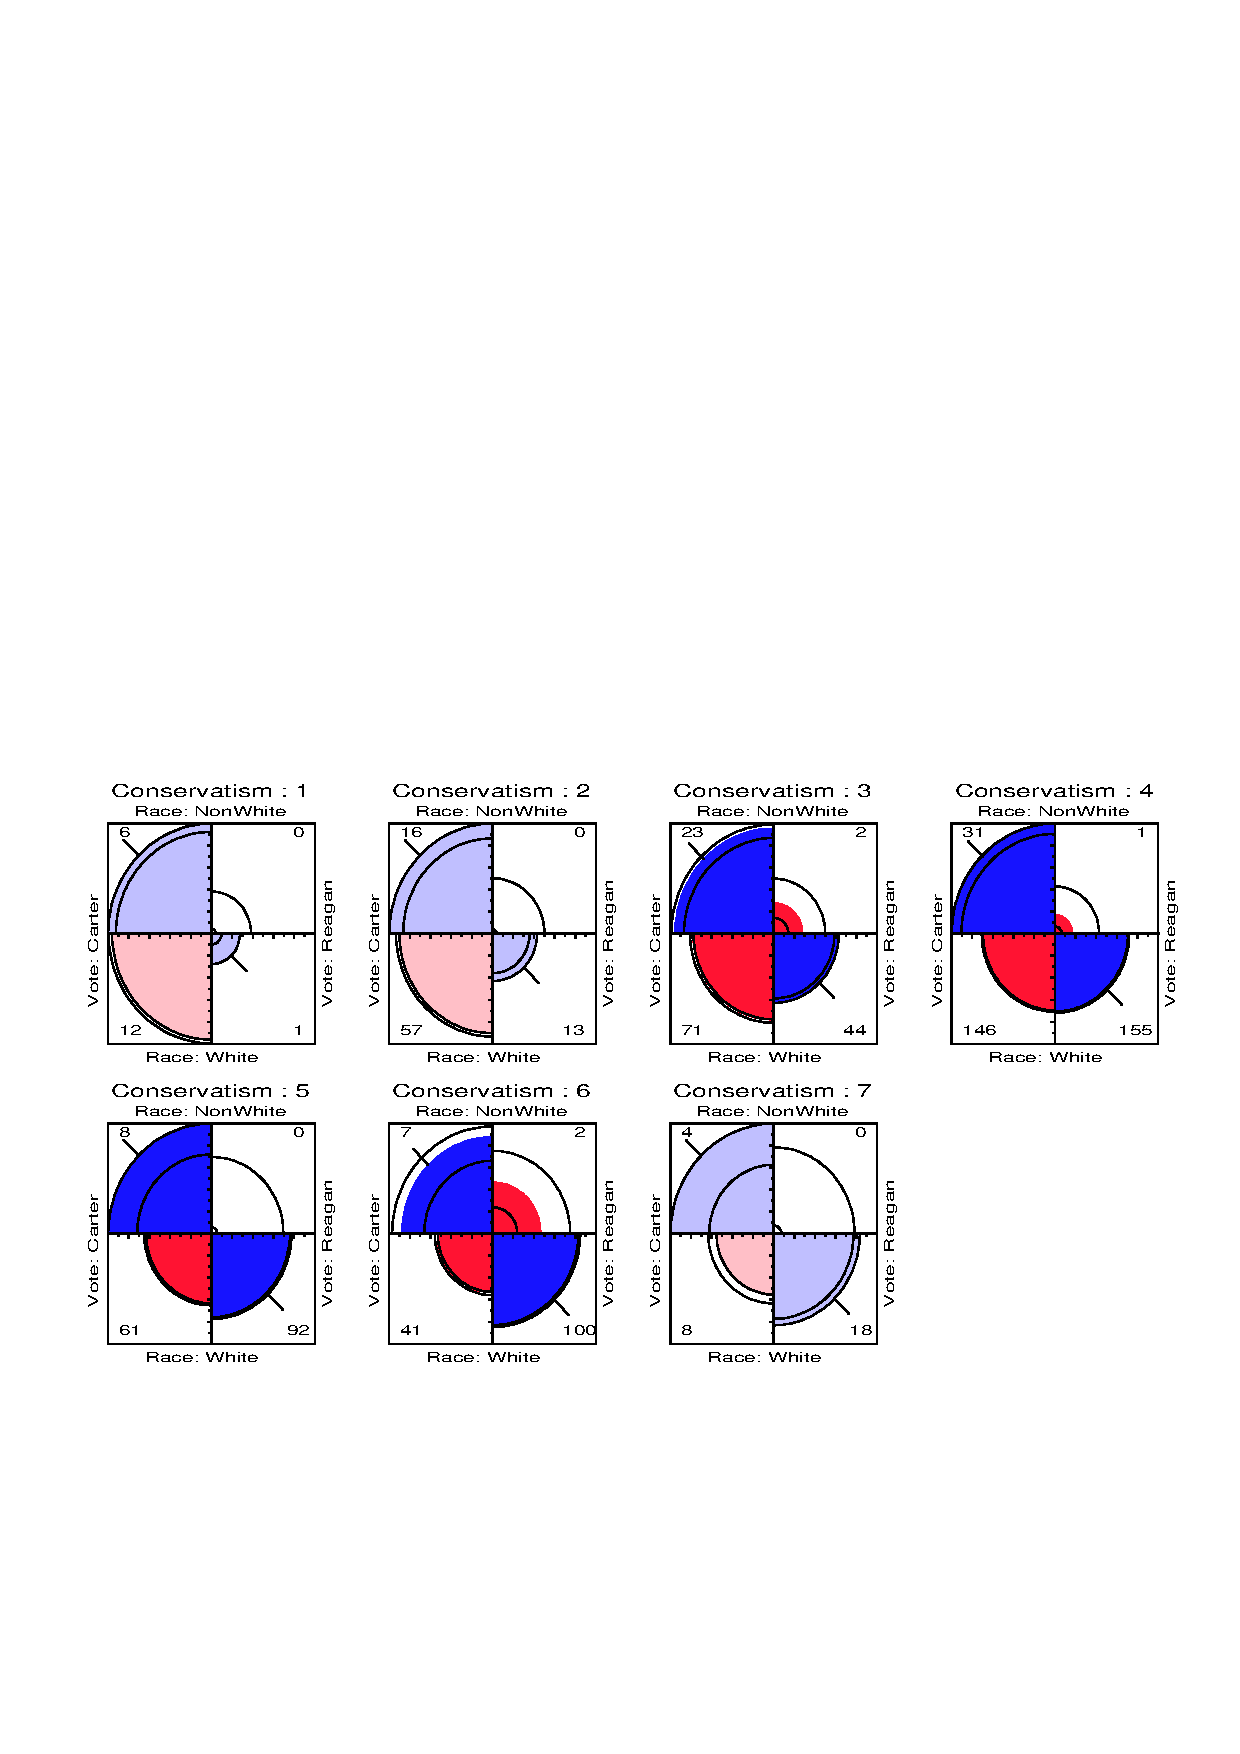
\includegraphics[width=\textwidth,clip]{reagan1a}
  \caption[Fourfold display for Vote, by Race and Conservatism]{Fourfold display for Vote, by Race and Conservatism, equating the number of White and Non White respondents at each level of Conservatism}%
  \label{fig:reagan1a}
\end{figure}

Thus, among Whites, in the bottom half of each panel,
we may compare the areas of the left and right quadrants,
and see that the propensity to vote for Reagan increases with
conservatism.
A similar trend is evident among Non White respondents, but there
are a number of zero frequencies here, among Non Whites who indicated they
voted for Reagan.

The conditional odds ratios for Vote and Race given Conservatism are all in the same direction, indicating that Whites were more likely to vote for
Reagan at \emph{any} level of Conservatism.
The \sasprog{fourfold}  gives the test of homogeneity of odds ratios
shown in \outref{out:reagan1.1},
which is equivalent to a test for lack-of-fit of the
homogeneous association \loglin\ model $[RC] [VR] [VC]$.
The tests of conditional independence, $V \perp R \given C$,
suggest that voting preference depends on race, and possibly conservatism.

\ixon{zero cells}
To illustrate the problem of zero cells, consider tests of fit of the
saturated model, $[RCV]$, and of the homogeneous association model,
$[RC] [VR] [VC]$, fit as \loglin\ models under three conditions:
\begin{seriate}
\item no adjustment for zeros,
\item replace zeros by $10^{-10}$, and
\item add 0.5 to each cell.
\end{seriate}
In each case, the models are fit
with the statements below, after possible adjustment to the \pname{count}
variable.
The results are summarized in \tabref{tab:reagzero}.
\begin{listing}
proc catmod data=vote;
   weight count;
   model cons*race*votefor = _response_ / ml noiter noresponse noprofile;
   loglin cons|race|votefor / title='Saturated model';
  run;
   loglin cons|race|votefor @2 / title='No 3-way association';
\end{listing}
In case (a), the four zero cell are treated as structural zeros, and
deleted, leaving only 2 df for the test of lack-of-fit in the
no-3-way model.
In case (b), the main effect parameter for Race cannot be estimated
and there is, paradoxically, 1 df for the test of the saturated model.
Case (c), adding 0.5 to each cell, has no anomalies, and we adopt this
solution for this example. In other cases it is recommended to compare
several approaches to determine if any conclusions are affected by
the presence of zero cells.
\ix{zeros!structural}

\begin{table}[htb]
 \caption{Effects of zero-cell actions on \loglin\ models for \pname{vote} data}\label{tab:reagzero}
 \begin{center}
 \begin{tabular}{l rrrr}
  \hline
   \multicolumn{1}{r}{Model:}  & \multicolumn{2}{c}{$[RCV]$} & \multicolumn{2}{c}{$[RC] [VR] [VC]$} \\
  Action                     & df & \GSQ\ & df & \GSQ\ \\ 
  \hline
(a)  None                       & 0 & . & 2 & 1.89 \\ 
(b)  $n=0 \rightarrow 10^{-10}$ & 1 & 0.00 & 6 & 4.96 \\ 
(c)  $n	\rightarrow n+\frac12$ & 0 & . & 6 & 3.45 \\ 
  \hline
 \end{tabular}
 \end{center}
\end{table}

\ixoff{zero cells}

\begin{Output}[htb]
\caption{Vote data: Test of Homogeneity of odds ratios}\label{out:reagan1.1}
\small
\verbatiminput{ch7/out/reagan1.1}
\end{Output}

We proceed to fit a main effects logit model.
Treating the vote for Reagan vs. Carter or other as the response, the
logit model with nominal main effects for race and conservatism is

\begin{equation} \label{eq:logrnom}
    \logit ( \mbox{Reagan} / \mbox{Carter} )  =
    \alpha   +
    \beta _i^{\mbox{\scriptsize Race}}  +
    \beta _j^{\mbox{\scriptsize Cons}}
	 \period
\end{equation}
Model \eqref{eq:logrnom} may be fit with \PROC{CATMOD} as follows. \begin{listing}
data vote;
    set vote;
    count = count + 0.5;
proc catmod data=vote order=data;
   weight count;
   response / out=predict;
   model votefor = race cons / noiter noresponse noprofile;
\end{listing}

The model fit statistics and parameter estimates for the logit model
\eqref{eq:logrnom} are shown in \outref{out:glogit1.1}.
The model fits quite well.
\begin{Output}[htb]
\caption{Vote data: Fit of the nominal main effects model}\label{out:glogit1.1}
\small
\verbatiminput{ch7/out/glogit1.1}
\end{Output}

To interpret the model, we plot the observed and predicted logits, with
90\% confidence intervals, as shown below.  The \macro{CATPLOT}
gives \figref{fig:glogit11}.
\begin{listing}
%pscale(lo=-5, hi=2.3, anno=pscale, prob=%str(0.01,.05,.1,.25,.5,.75,.9));

axis1 order=(-5 to 2) offset=(0,3)
      label=(a=90 'Logit (Reagan / Carter)');
axis2 label=('Conservatism') offset=(2);
symbol1 i=none v=circle h=1.9 c=black;
symbol2 i=none v=square h=1.7 c=red  ;
legend1 position=(bottom inside center) offset=(,2);
%catplot(data=predict, class=race, x=cons, z=1.65, anno=pscale,
   legend=legend1);
\end{listing}

%% one figure
\begin{figure}[htb]
  \centering
  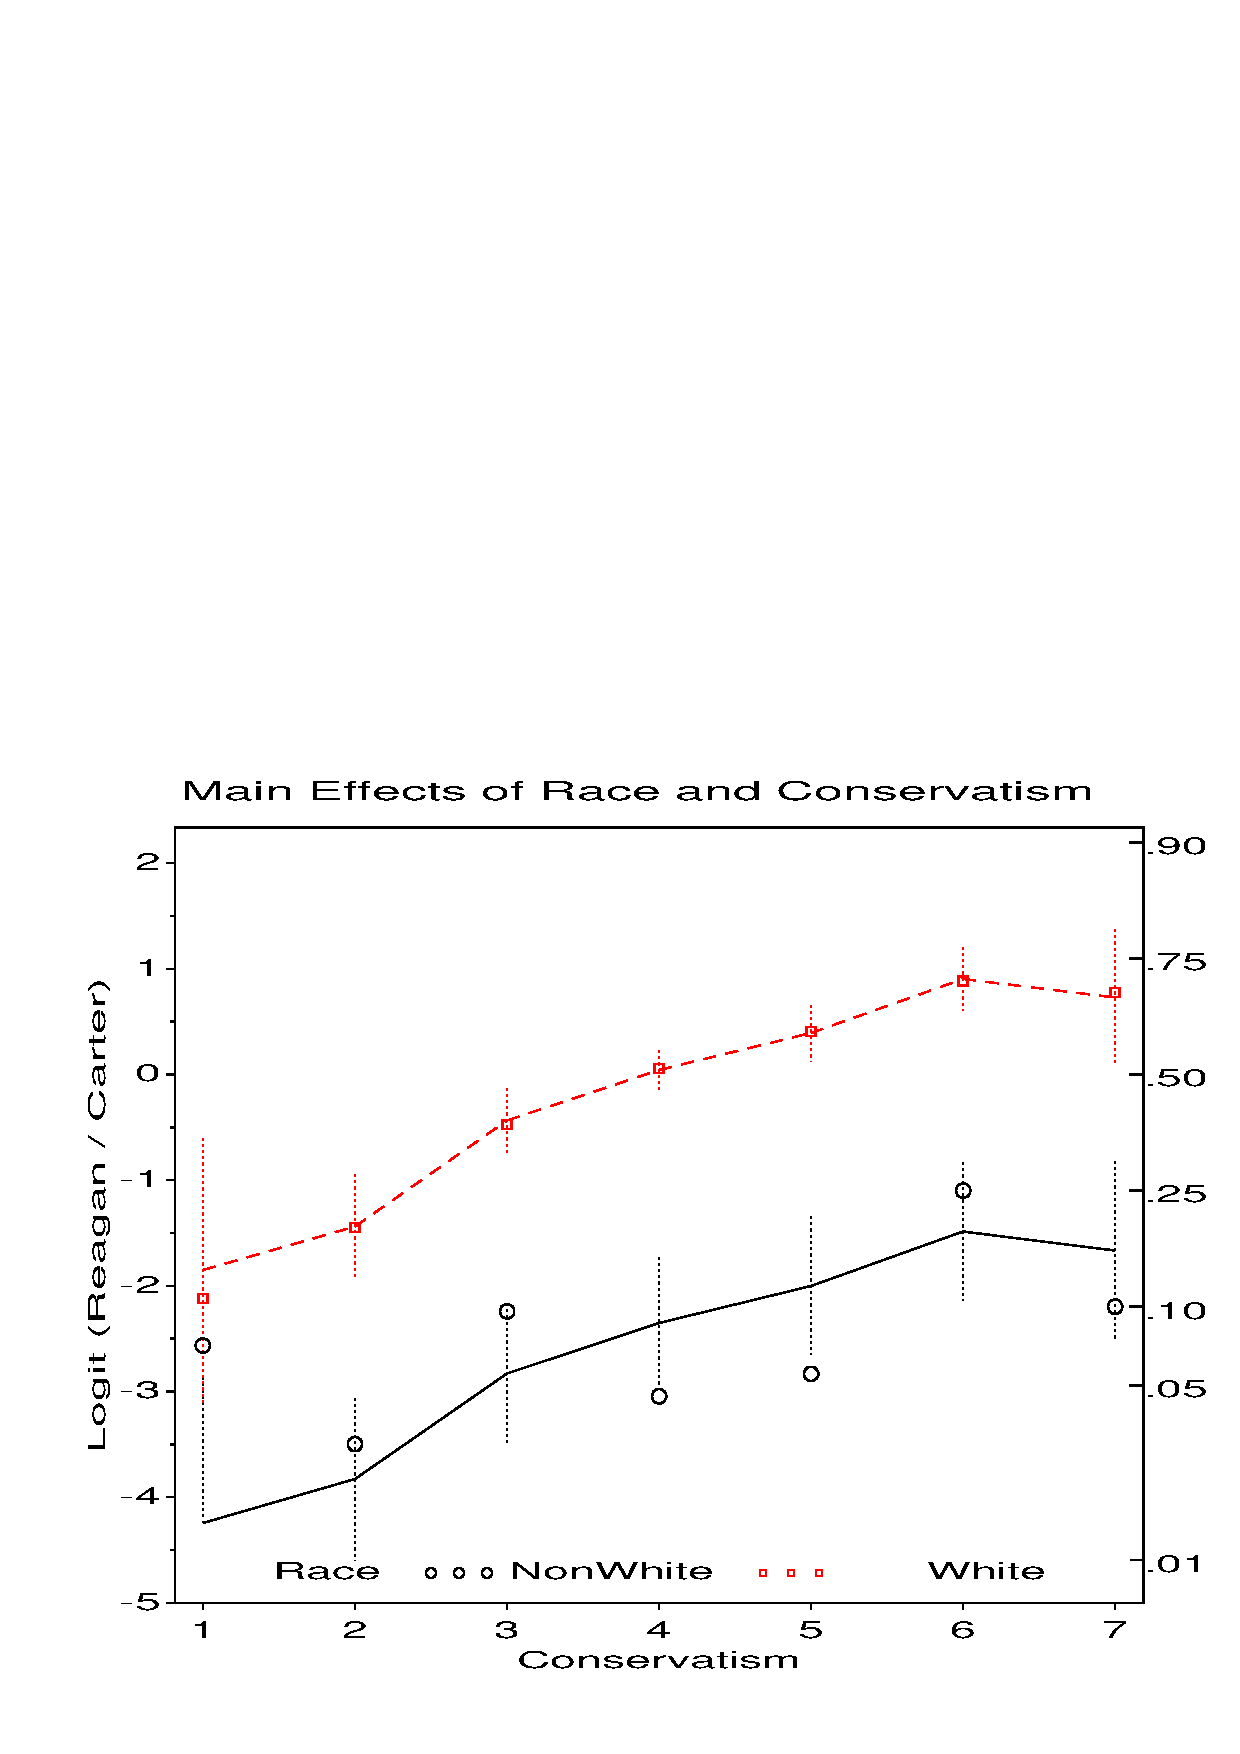
\includegraphics[scale=.6]{glogit11}
  \caption[Observed and fitted logits for main effects model]{Observed (points) and fitted (lines) logits for main effects model.  Dotted lines show a 90\% confidence interval around the predicted log odds.}%
  \label{fig:glogit11}
\end{figure}
Notice that for both Whites and Non Whites, the log odds of voting for
Reagan increases with conservatism.  This is also reflected in the
parameter estimates for \pname{cons} in \outref{out:glogit1.1},
which increase in approximately equal steps.
Model \eqref{eq:logrnom} does not use the ordinal nature of conservatism.
A model which uses conservatism as a direct,
quantitative independent variable ($c$) can be expressed as

\begin{equation} \label{eq:logrlin}
  \mbox{logit ( Reagan / Carter )}  =
  \alpha   +
  \beta _i^{\mbox{\scriptsize Race}}  +
  \beta ^{\mbox{\scriptsize Cons}} \,  c
\end{equation}
Note that there is just one parameter for conservatism,
$ \beta ^{\mbox{\scriptsize Cons}}$, which is interpreted as
an increase in the log odds of a vote for Reagan for each
change of 1 unit in conservatism.
Model \eqref{eq:logrlin} may be fit with \PROC{CATMOD}
just by adding the statement \pname{DIRECT CONS;}
\begin{listing}
proc catmod data=vote order=data;
   direct cons;
   weight count;
   response / out=predict;
   model votefor = race cons / noiter noresponse noprofile ;
   title 'Linear Effect for Conservatism' h=2.5 a=-90 ' ';
\end{listing}
The \LR\ \GSQ\ for this model is $\GSQ (11) = 9.58$, and
the difference in \GSQ\ for Models
\eqref{eq:logrlin} and \eqref{eq:logrnom} is
$\Delta \GSQ (5) = 6.13$,
so the linear model cannot be rejected, given that the nominal
model fits.  The estimate $\widehat{\beta} ^{\mbox{\scriptsize Cons}} = 0.472$
indicates that the odds of voting for Reagan increase by a factor of
$\exp(0.472) = 1.60$ (60\%) for each step of increasing conservatism.

%\begin{Output}[htb]
%\caption{}\label{out:glogit1.2}
%\small
%\verbatiminput{ch7/out/glogit1.2}
%\end{Output}

The observed and fitted logits are plotted exactly as before, using
the same \macro{CATPLOT} call with the new \ODS\ \pname{predict}.
The plot is shown in \figref{fig:glogit12}.
Note that the 90\% confidence limits around predicted values are
noticeably smaller than in \figref{fig:glogit11}.
This is but one advantage of models for ordinal variable,
which we discuss in the following section.
%% one figure
\begin{figure}[htb]
  \centering
  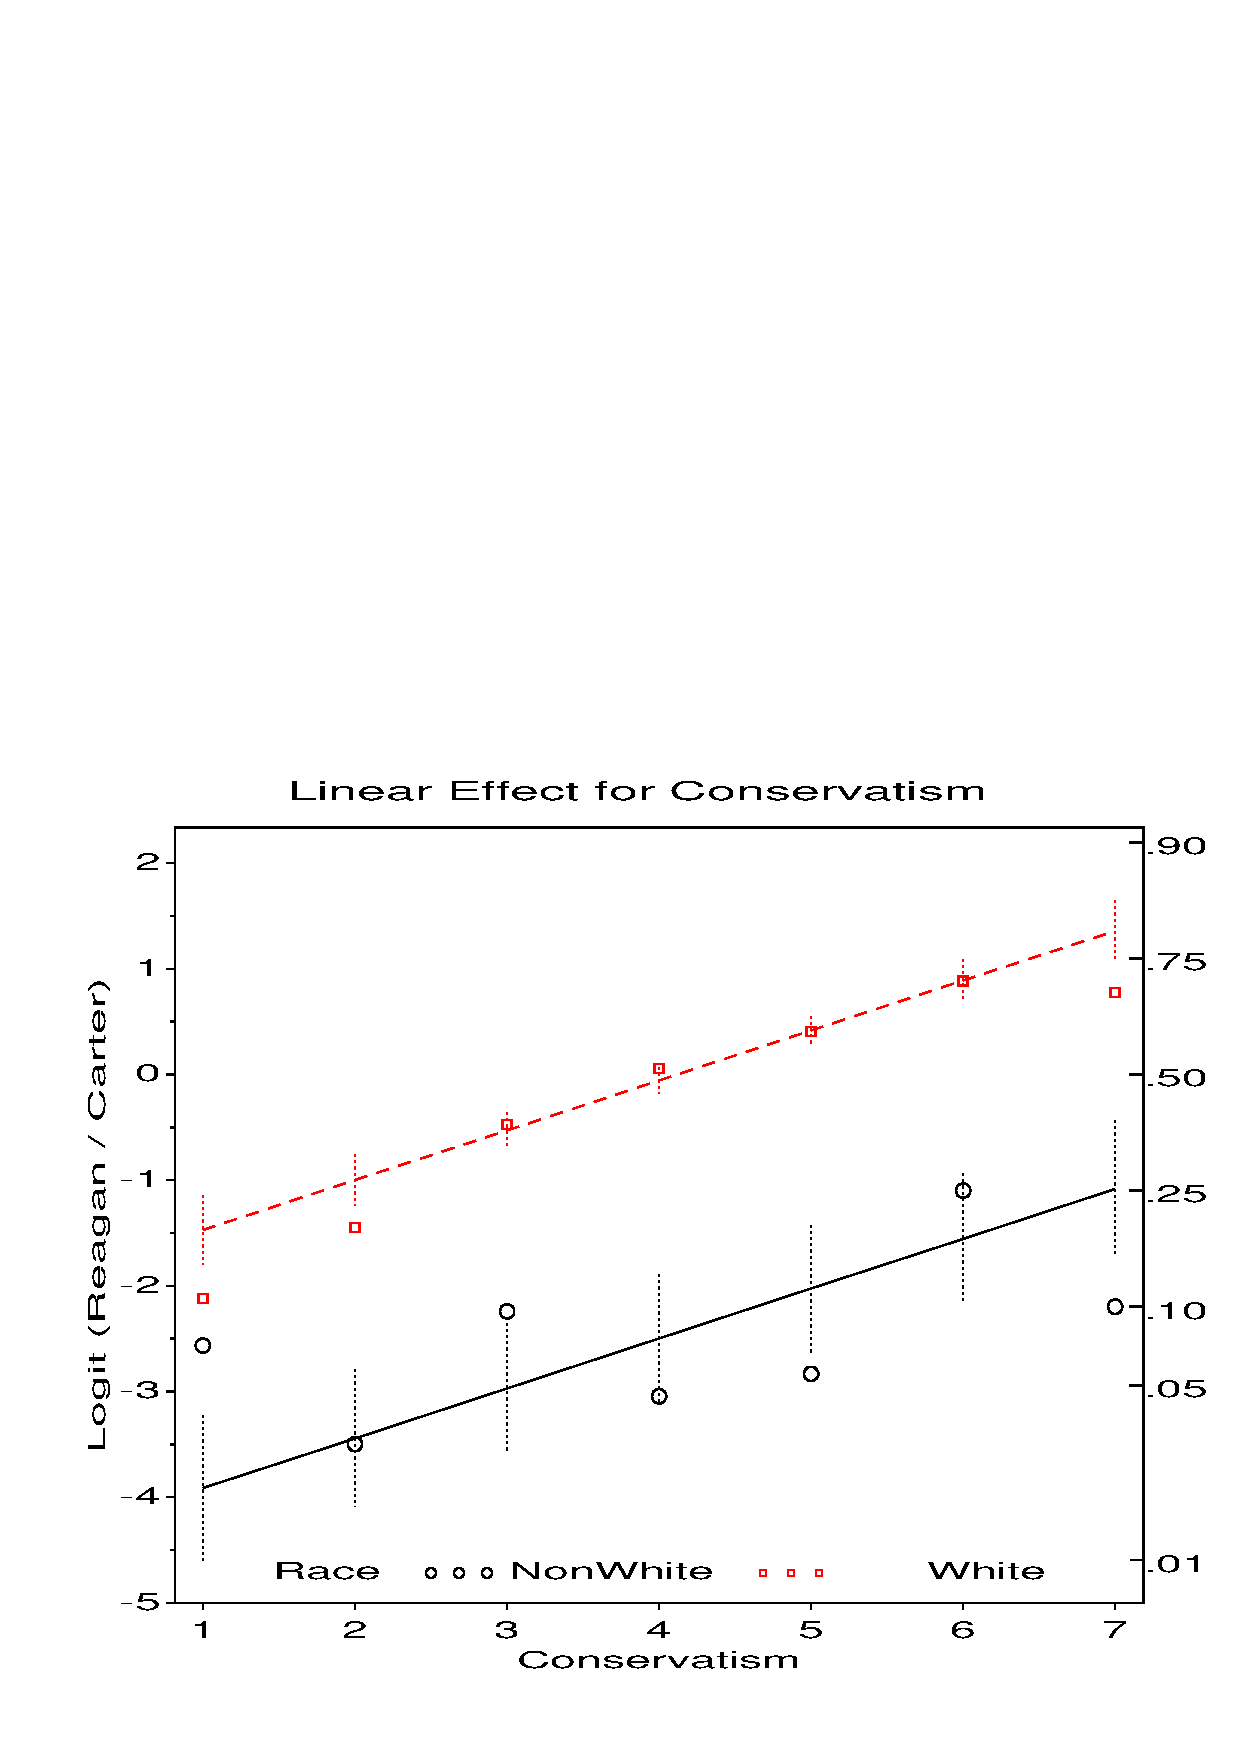
\includegraphics[scale=.6]{glogit12}
  \caption[Observed and fitted logits for linear effect of conservatism]{Observed (points) and fitted (lines) logits for linear effect of conservatism.  Dotted lines show a 90\% confidence interval around the predicted log odds.}%
  \label{fig:glogit12}
\end{figure}
\end{Example}

